{\emph {Finally, we now study the latency of rule deletions}}.
We again use bursts of operations.
$T(r_i)$ denotes the time we stop observing packets matching rule $r_i$
from the intended port of the rule action. We define deletion latency
as $T(r_i)-T(r_{i-1})$.

\begin{figure*}[!t]
	\centering
        \begin{subfigure}[b]{0.40\textwidth}
                \centering
		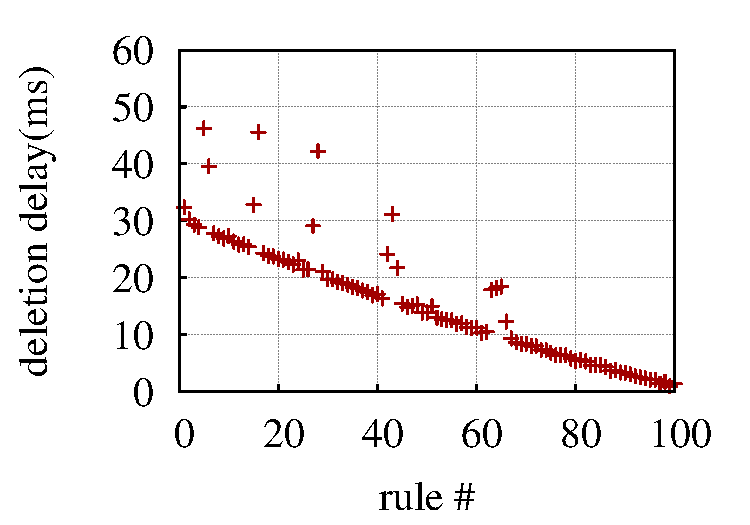
\includegraphics[width=\textwidth]{./figures/mazu/jan27_bcm_del_same_burst_100-eps-converted-to.pdf}
		\caption{100 rules in table}
		\label{fig:bcm_del_same_burst_100}
	\end{subfigure}
        \begin{subfigure}[b]{0.40\textwidth}
                \centering
		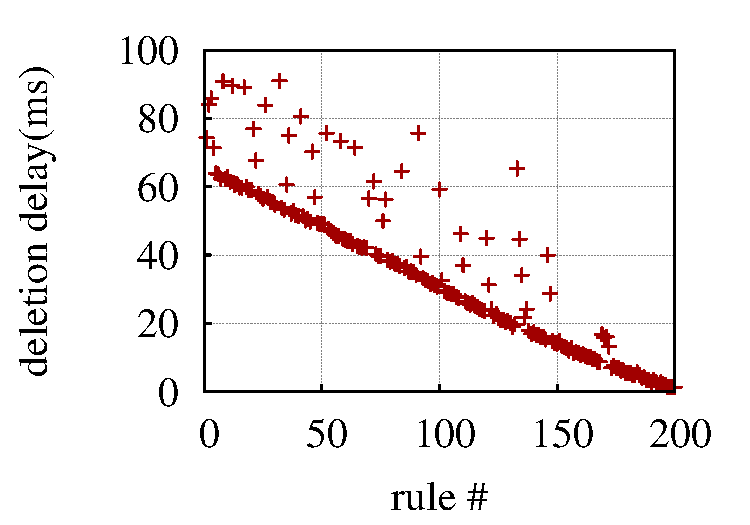
\includegraphics[width=\textwidth] {./figures/mazu/jan27_bcm_del_same_burst_200-eps-converted-to.pdf}
		\caption{200 rules in table}
		\label{fig:bcm_del_same_burst_200}
	\end{subfigure}
	\caption{ {\bf \BroadcomOne} per-rule {\bf del.} latency, same priority}
	\label{fig:occupancy-broadcom-deletion}
\end{figure*}

\begin{figure*}[!t]
	\centering
        \begin{subfigure}[b]{0.40\textwidth}
                \centering
		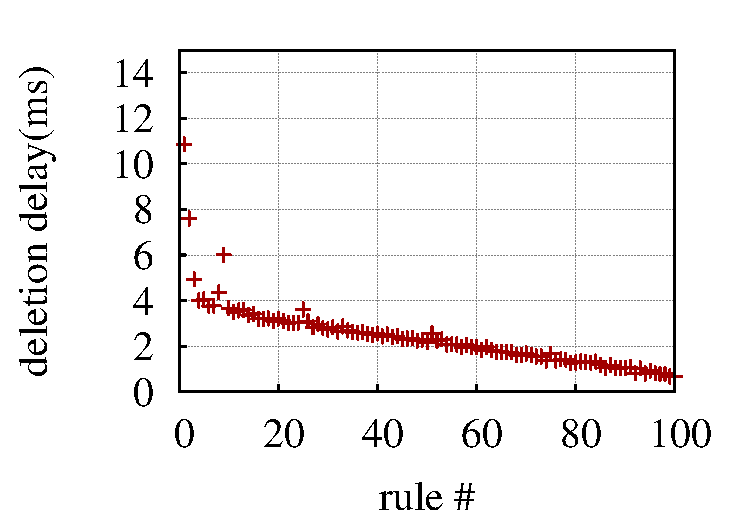
\includegraphics[width=\textwidth]{./figures/mazu/jan27_intel_del_same_burst_100-eps-converted-to.pdf}
		\caption{100 rules in table}
		\label{fig:intel_del_same_burst_100}
	\end{subfigure}
        \begin{subfigure}[b]{0.40\textwidth}
                \centering
		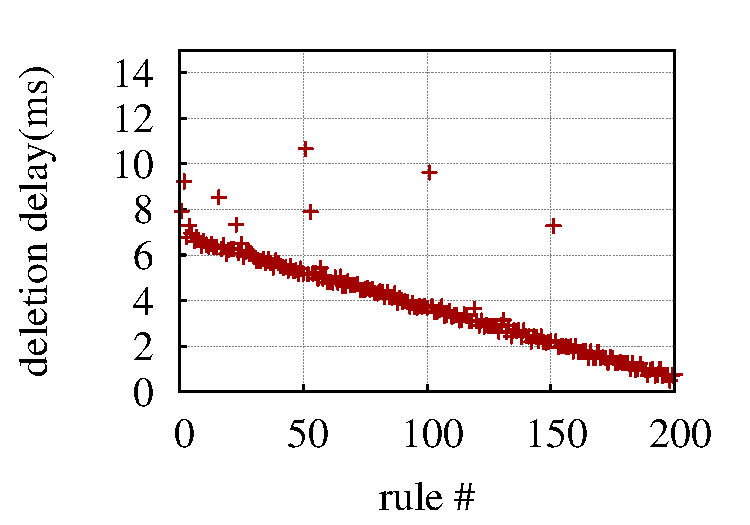
\includegraphics[width=\textwidth]{./figures/mazu/jan27_intel_same_burst_200-eps-converted-to.pdf}
		\caption{200 rules in table}
		\label{fig:intel_del_same_burst_200}
	\end{subfigure}
	\caption{{\bf \Intel} per-rule {\bf del.} latency, same priority}
	\label{fig:occupancy-intel-deletion}
\end{figure*}

\tightparagraph{Table Occupancy} We pre-insert $S$ rules into a switch, all with
the same priority. We then delete one rule at a time, sending deletion
requests back-to-back. The results for \BroadcomOne at $S=100$ and $S=200$
are shown in \figsref{fig:bcm_del_same_burst_100}{fig:bcm_del_same_burst_200},
respectively. We see that per rule deletion delay decreases as the table occupancy drops. We see a similar trend for Intel (\figsref{fig:intel_del_same_burst_100}{fig:intel_del_same_burst_200}) \BroadcomThree and \IBM (not shown).


\begin{figure*}[!t]
	\centering
        \begin{subfigure}[b]{0.40\textwidth}
                \centering
		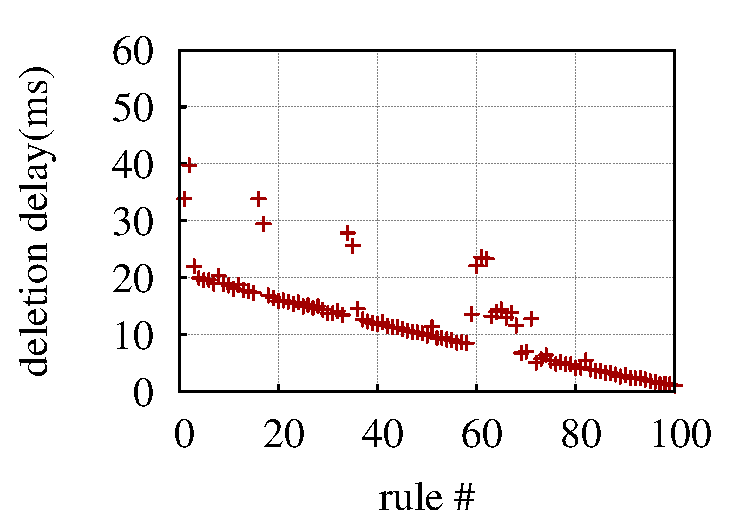
\includegraphics[width=\textwidth]{./figures/mazu/jan27_bcm_del_incr_burst_100-eps-converted-to.pdf}
		\caption{increasing priority}
		\label{fig:bcm_del_incr_burst_100}
	\end{subfigure}
        \begin{subfigure}[b]{0.40\textwidth}
                \centering
		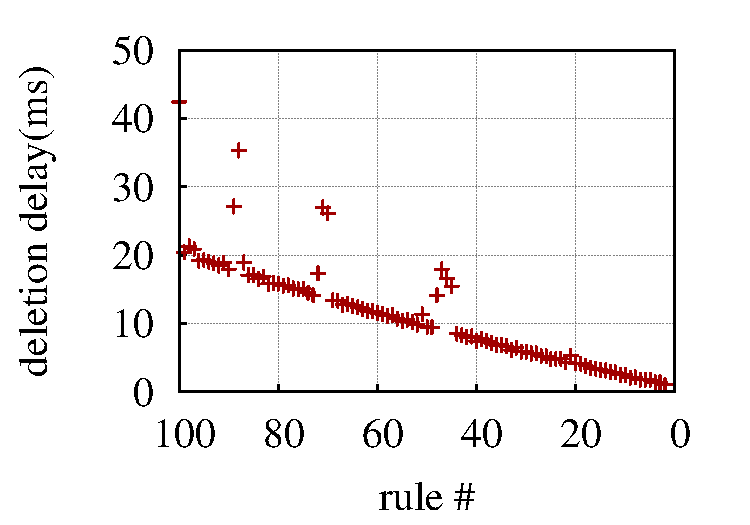
\includegraphics[width=\textwidth]{./figures/mazu/jan27_bcm_del_decr_burst_100-eps-converted-to.pdf}
		\caption{decreasing priority}
		\label{fig:bcm_del_decr_burst_100}
	\end{subfigure}
	\caption{{\bf \BroadcomOne} priority per-rule {\bf del.} latency, 
    B=100}
	\label{fig:priority-broadcom-deletion}
\end{figure*}

\begin{figure*}[!t]
	\centering
        \begin{subfigure}[b]{0.40\textwidth}
                \centering
		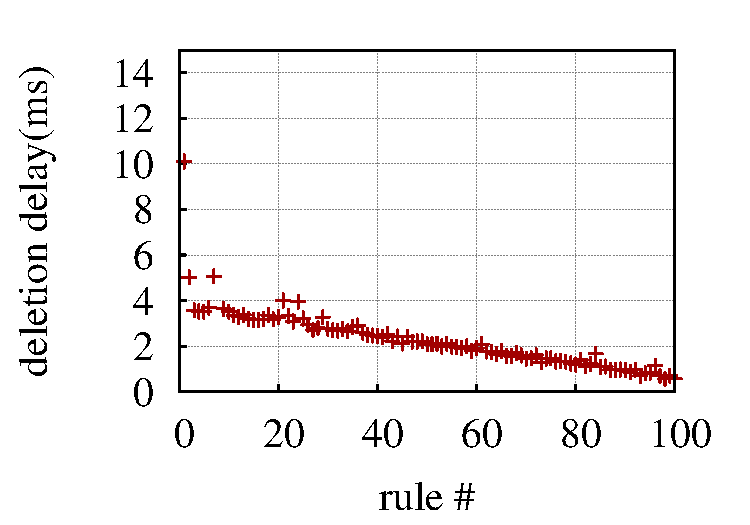
\includegraphics[width=\textwidth]{./figures/mazu/jan27_intel_del_incr_burst_100-eps-converted-to.pdf}
		\caption{increasing priority}
		\label{fig:intel_del_incr_burst_100}
	\end{subfigure}
        \begin{subfigure}[b]{0.40\textwidth}
                \centering
		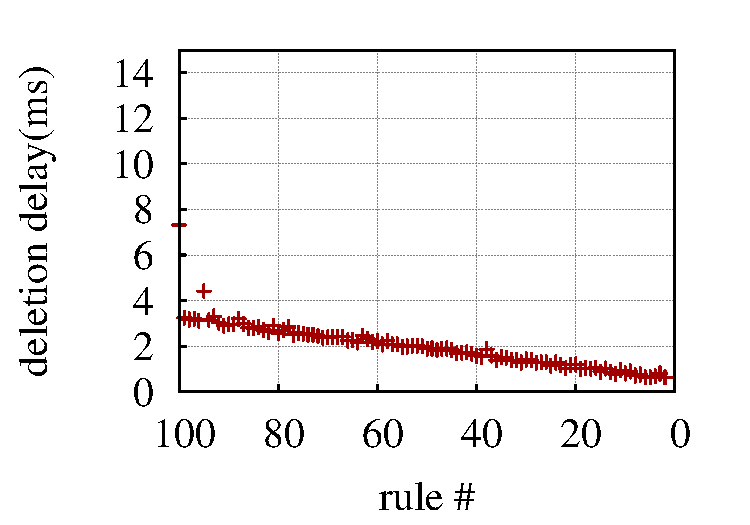
\includegraphics[width=\textwidth]{./figures/mazu/jan27_intel_del_decr_burst_100-eps-converted-to.pdf}
		\caption{decreasing priority}
		\label{fig:intel_del_decr_burst_100}
	\end{subfigure}
	\caption{{\bf Intel} priority per-rule {\bf del.} latency, B=100}
	\label{fig:priority-intel-deletion}
\end{figure*}


\tightparagraph{Rule Priorities} We start with $B$ existing rules in the switch, 
and delete one rule at a time
in increasing and decreasing priority order. 
For all switches (\BroadcomOne and \Intel shown in
\figsref{fig:priority-broadcom-deletion}{fig:priority-intel-deletion},
respectively)
deletion is not affected by the priorities of rules in the table or the order 
of deletion.

\tightparagraph{\bf Root cause} Since deletion delay decreases with rule number 
in all cases, we conclude that deletion is incurring TCAM reordering.
We also observe that processing rule timeouts at the switch does not
noticeably impact \flowmod operations. Given these two observations, we
recommend allowing rules to time out rather than explicitly deleting them, if
possible.

